% Provenance (never printed): old terminale S material on magmatism in
% subduction zones (volcanic arcs above the slab, water released by the slab
% and hydrous melting of the mantle wedge, andesitic volcanism and granitoid
% plutons, growth of the continental crust). Owner (Sync 0): volcanic arc,
% hydrous melting, granodiorite, batholith, continental growth. Subduction,
% slab, Wadati-Benioff zone, blueschist and eclogite are g11.06's; partial and
% decompression melting and peridotite g11.05's; andesite, diorite, rhyolite,
% pluton g11.08's; continental crust g12.01's; magma, explosive eruption Book 1's
% (g7): recalled, never redefined. Figures: figdata/grade-12/arc_magmatism.py
% (GVP volcanoes, ComCat NE Japan band, dry solidus via grade-11
% geotherm_solidus.py, wet solidus brackets of Wang 2020 and Kawamoto-Holloway 1997).
\chapter{Magmatisme di Zona Subduksi}\label{ch:g12:subduction-magmatism}

Pada 18 Mei 1980, pukul 8.32 pagi, gempa bumi bermagnitudo 5.1 mengguncang
Gunung St.~Helens. Seketika lereng utara gunung api itu, yang telah menggembung
ke luar sekitar dua meter sehari, longsor: longsoran puing terbesar dalam
sejarah yang tercatat, sekitar \qty{2.5}{km^3} batuan. Terbebas dari bebannya,
magma kaya gas di dalamnya menyembur ke samping melalui bekas longsoran itu,
dengan kecepatan tidak kurang dari \qty{480}{km/h}, merobohkan hutan seluas
\qty{600}{km^2}. Dalam lima belas menit, sebuah kolom abu menjulang lebih dari
\qty{24}{km}, dan letusan itu berlangsung selama sembilan jam. Enam puluh satu
orang tewas atau tidak pernah ditemukan.
% ledger: usgs:b2-msh-1980, usgs:msh-deaths

\begin{omfigure}
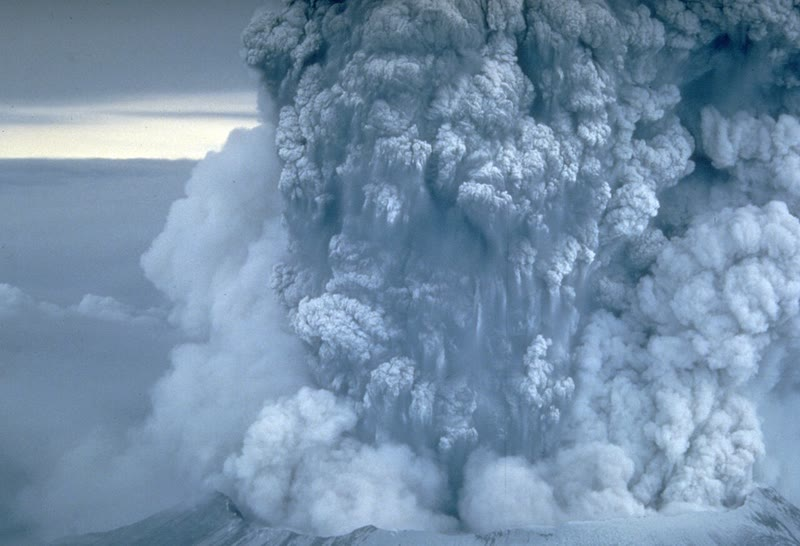
\includegraphics[width=0.55\linewidth]{images/book2/g12-swanson-st-helens-plume.jpg}

{\small Kolom abu Gunung St.~Helens pada 18 Mei 1980, yang naik lebih dari
\qty{24}{km} dalam waktu kurang dari lima belas menit. Foto Donald
A.~Swanson, USGS (domain publik).}
\end{omfigure}
% ledger: photo:g12-st-helens, usgs:b2-msh-1980

Gunung St.~Helens adalah salah satu dari sederet gunung api --- Baker, Rainier,
Hood, Shasta, dan lainnya --- yang berdiri di atas tempat sebuah lempeng samudra
yang kecil, lempeng Juan de Fuca, tenggelam di bawah Amerika Utara. Bab ini
menanyakan mengapa gunung-gunung api dijumpai di sana, mengapa letusannya begitu
sering dahsyat, dan apa yang terjadi pada magma yang tidak pernah mencapai
permukaan.
% ledger: earle:cascades

\begin{recall}
Di \omterm{def:g11:subduction-zones:subduction}{zona subduksi}, lempeng \omterm{def:g11:ocean-ridges:oceanic-lithosphere}{litosfer samudra} tenggelam kembali ke dalam mantel di
bawah lempeng lain; gempa-gempa buminya, yaitu \omterm{def:g11:subduction-zones:benioff}{zona Wadati--Benioff}, menelusuri
\omterm{def:g11:subduction-zones:slab}{lempengan} itu sampai sedalam \qty{670}{km} (\cref{ch:g11:subduction-zones}).
Mantel tersusun dari \omterm{def:g11:ocean-ridges:peridotite}{peridotit}; mantel itu padat, tetapi batuan yang naik dan
kurang terjepit dapat meleleh sebagian, melalui \omterm{def:g11:ocean-ridges:partial-melting}{pelelehan dekompresi}, seperti di
bawah punggungan (\cref{ch:g11:ocean-ridges}). \omterm{def:g11:igneous-rocks:rock-names}{Andesit} adalah \omterm{def:g11:igneous-rocks:volcanic-plutonic}{batuan vulkanik}
di antara basalt dan \omterm{def:g11:igneous-rocks:rock-names}{riolit}, \omterm{def:g11:igneous-rocks:rock-names}{diorit} padanan \omterm{def:g11:igneous-rocks:volcanic-plutonic}{plutoniknya}, dan \omterm{def:g11:igneous-rocks:intrusion}{pluton} adalah tubuh
magma besar yang mendingin di bawah tanah (\cref{ch:g11:igneous-rocks}). \omterm{def:g12:continental-crust:continental-crust}{Kerak
benua} tebal dan ringan, dengan bagian atas yang sebagian besar berupa batuan
granitik (\cref{ch:g12:continental-crust}). Letusan eksplosif menghancurkan
magma menjadi kepingan-kepingan oleh gasnya sendiri (Buku 1, kelas 7).
\end{recall}
% ledger: tulane:magma-types, tulane:intrusions, rg14:crust

\section{Busur gunung api}

Sebagian besar gunung api aktif di darat tidak berdiri secara acak. Dari 1214
gunung api yang telah meletus sejak akhir zaman es terakhir dan tercantum dalam
katalog Global Volcanism Program, 838 --- lebih dari dua dari tiga --- berdiri di
atas \omterm{def:g11:subduction-zones:subduction}{zona subduksi}. Di sekeliling Pasifik, gunung-gunung api itu membentuk
lingkaran yang hampir tidak terputus, yang sering disebut Cincin Api, dan setiap
deretnya sejajar dengan sebuah palung, di sisi lempeng yang tidak tenggelam.
% values: n_volcanoes 1214, n_subduction 838, frac_subduction 0.690 (arc_magmatism.py)
% ledger: data:gvp, tulane:arc

\begin{omfigure}
\begin{tikzpicture}
\begin{axis}[ommap, width=\linewidth, xtick={-180,-90,...,180}, ytick={-60,0,60},
  legend style={font=\scriptsize, at={(0.5,-0.13)}, anchor=north, legend columns=3,
    /tikz/every even column/.append style={column sep=6pt}}]
\addplot[fill=omLithAlluv, draw=black!45, line width=0.2pt, forget plot] table {figdata/out/shared-geo-land.dat};
\addplot[black!70, line width=0.5pt, forget plot] table {figdata/out/shared-geo-school-subduction.dat};
\addplot[fill=black!70, draw=none, forget plot] table {figdata/out/shared-geo-school-teeth.dat};
% computed in figdata/grade-12/arc_magmatism.py; ledger: data:gvp, data:pb2002, data:ne-land
\addplot[only marks, mark=triangle*, mark size=1.1pt, black!40] table[x=lon, y=lat] {figdata/out/grade-12-arc_magmatism-world-other.dat};
\addplot[only marks, mark=triangle*, mark size=1.3pt, omThm] table[x=lon, y=lat] {figdata/out/grade-12-arc_magmatism-world-sub.dat};
\addlegendimage{black!70, line width=0.5pt}
\legend{{gunung api lain}, {gunung api di atas zona subduksi}, {palung}}
\end{axis}
\end{tikzpicture}

{\small Gunung-gunung api yang aktif sejak akhir zaman es terakhir, merah bila
berdiri di atas \omterm{def:g11:subduction-zones:subduction}{zona subduksi}, beserta palung-palung (garis hitam, segitiga pada
lempeng yang berada di atas). Data: Smithsonian Global Volcanism Program; batas
lempeng dari Bird (2003); daratan dari Natural Earth.}
\end{omfigure}
% values: n_subduction 838 of 1214 (arc_magmatism.py)

\begin{definition}[Busur gunung api]\label{def:g12:subduction-magmatism:arc}
Yang disebut \emph{busur gunung api}\index{busur gunung api} adalah deretan
gunung api pada lempeng yang berada di atas di sebuah \omterm{def:g11:subduction-zones:subduction}{zona subduksi}, sejajar
dengan palung, yang berdiri di atas tempat \omterm{def:g11:subduction-zones:slab}{lempengan} telah mencapai kedalaman
sekitar seratus kilometer. Busur itu disebut \emph{busur kepulauan} bila muncul
dari dasar laut, seperti di Jepang atau Indonesia, dan busur benua bila berdiri
di atas benua, seperti di Andes atau Cascade.
\end{definition}
% ledger: tulane:arc, earle:arc-water, earle:cascades, sa06:slab-depth

Tepi busur yang paling dekat dengan palung disebut \textbf{front vulkanik}: di
sisi palung dari front itu, sama sekali tidak ada gunung api. Seberapa dalam
\omterm{def:g11:subduction-zones:slab}{lempengan} di bawahnya?

\begin{proposition}[Lempengan di bawah front vulkanik]\label{prop:g12:subduction-magmatism:depth}
Bila \omterm{def:g11:subduction-zones:slab}{lempengan} itu sebuah bidang yang miring dengan sudut $\theta$ dari palung,
dan front vulkanik terletak pada jarak mendatar $d$ dari palung, maka bagian
atas \omterm{def:g11:subduction-zones:slab}{lempengan} terletak di bawah front itu pada kedalaman
\[
  H = d \tan\theta .
\]
\end{proposition}

\begin{proof}
Ambillah penampang tegak yang melintasi palung. \omterm{def:g11:subduction-zones:slab}{Lempengan}, permukaan, dan garis
tegak di bawah front membentuk segitiga siku-siku, dengan sudut siku-siku di
bawah front: sisi di sepanjang permukaan adalah $d$, sisi tegaknya adalah
$H$, dan sudut di palung adalah $\theta$. Jadi $\tan\theta = H/d$.
\end{proof}

Sebuah kompilasi atas 839 pusat gunung api di sepanjang \qty{33000}{km} busur
mengukur $H$ di bawah masing-masing pusat itu: dirata-ratakan atas
bentangan-bentangan busur sepanjang \qty{500}{km}, nilainya berkisar dari 72
sampai \qty{173}{km}, dengan rata-rata \qty{105}{km}. Busur di atas \omterm{def:g11:subduction-zones:slab}{lempengan}
yang curam terletak dekat dengan palungnya, busur di atas \omterm{def:g11:subduction-zones:slab}{lempengan} yang landai
jauh darinya, tetapi \omterm{def:g11:subduction-zones:slab}{lempengan} di bawahnya selalu berada sekitar seratus
kilometer di bawah permukaan.
% ledger: sa06:slab-depth

\begin{method}[Mencari lempengan di bawah gunung api]\label{met:g12:subduction-magmatism:slab}
\begin{enumerate}
  \item Ambillah gempa-gempa bumi dalam sebuah pita sempit yang melintasi
        busur, dan plotkan kedalamannya terhadap jaraknya melintasi pita itu,
        menurut skala yang sebenarnya.
  \item Pertahankan gempa bumi yang lebih dalam dari sekitar \qty{70}{km}:
        gempa yang lebih dangkal juga terjadi di lempeng yang berada di atas
        dan pada sesar di antara kedua lempeng.
  \item Gambarlah garisnya, atau bacalah kedalamannya, dari gempa-gempa dalam
        di bawah front vulkanik: itulah kedalaman \omterm{def:g11:subduction-zones:slab}{lempengan} di sana.
  \item Periksalah dengan $H = d\tan\theta$, dengan mengukur $d$ dari palung
        dan kemiringan $\theta$ pada penampang.
\end{enumerate}
\end{method}

\begin{omfigure}
\begin{tikzpicture}
\begin{axis}[omsection, name=jp, scale only axis, width=0.8\linewidth, height=0.2857\linewidth,
  xmin=0, xmax=700, ymin=0, ymax=250, y dir=reverse,
  xlabel={jarak di timur \ang{138}~BT (\unit{km})}, ylabel={kedalaman (\unit{km})},
  xtick={0,100,...,700}, ytick={0,50,...,250}, tick label style={font=\small},
  every axis label/.append style={font=\small}]
% computed in figdata/grade-12/arc_magmatism.py; ledger: data:b2-usgs-ne-japan, data:gvp, data:pb2002
\addplot[only marks, mark=*, mark size=0.55pt, black!35] table[x=x_km, y=depth] {figdata/out/grade-12-arc_magmatism-jp-quakes.dat};
\addplot[omDef, line width=0.9pt, dashed] table[x=x_km, y=depth] {figdata/out/grade-12-arc_magmatism-jp-slab.dat};
\addplot[only marks, mark=triangle*, mark size=2.6pt, omThm] table[x=x_km, y expr=-7] {figdata/out/grade-12-arc_magmatism-jp-volc.dat};
\draw[omThm, densely dotted, line width=0.8pt] (axis cs:259.2,0) -- (axis cs:259.2,98.2);
\fill[omThm] (axis cs:259.2,98.2) circle (1.6pt);
\coordinate (front) at (axis cs:259.2,-14);
\coordinate (trench) at (axis cs:528.9,-14);
\coordinate (H) at (axis cs:262,60);
\coordinate (slab) at (axis cs:95,228);
\draw[black, line width=0.9pt] (axis cs:528.9,-12) -- (axis cs:528.9,0);
\end{axis}
\node[font=\scriptsize, anchor=south, text=omThm] at (front) {front vulkanik (Iwate)};
\node[font=\scriptsize, anchor=south] at (trench) {Palung Jepang};
\node[font=\scriptsize, anchor=west, text=omThm, fill=white, inner sep=1pt] at (H) {\qty{98}{km}};
\node[font=\scriptsize, anchor=west, text=omDef, fill=white, inner sep=1pt] at (slab) {lempengan, miring sekitar \ang{20}};
\end{tikzpicture}

{\small Penampang yang melintasi Jepang timur laut menurut skala yang sebenarnya:
gempa-gempa bumi bermagnitudo 4.5 atau lebih antara \ang{37.5} dan
\ang{40.5}~LU, 1976--2025 (kelabu), gunung-gunung api dalam pita yang sama
(segitiga merah), dan garis yang dicocokkan pada gempa-gempa bumi yang lebih
dalam dari \qty{70}{km} (biru, putus-putus). Dua dari lima gempa dangkal di
timur \ang{141.5}~BT berasal dari tahun 2011, tahun gempa bumi besar bulan
Maret. Data: katalog gempa bumi
USGS; Smithsonian Global Volcanism Program; batas lempeng
dari Bird (2003).}
\end{omfigure}
% values: shallow (<70 km) events east of 141.5 E: 3622, of which 1451 in 2011 (0.40); ledger usgs:tohoku
% values: jp_front_lon 141.0 (x 259.2 km), jp_trench_lon 144.12 (x 528.9), jp_front_trench_km 269.4, jp_dip_deg 19.98, jp_H_geom 98.0, bin_141_median 98.15, jp_slab_depth_front 105.6 (arc_magmatism.py)

\begin{example}[Jepang timur laut]\label{ex:g12:subduction-magmatism:japan}
Dalam pita pada gambar itu, gunung api yang paling timur adalah Iwate, pada
\ang{141.0}~BT, dan Palung Jepang terletak pada \ang{144.1}~BT. Satu derajat
bujur di sana adalah
$111.2\cos\ang{39} \approx \qty{86.4}{km}$, sehingga $d \approx 3.12 \times 86.4
\approx \qty{270}{km}$. Gempa-gempa dalam miring sekitar \ang{20}, dan
\[
  H = 270 \times \tan\ang{20} \approx \qty{98}{km}.
\]
Gempa-gempa bumi yang lebih dalam dari \qty{70}{km} yang terletak tepat di
bawah front mempunyai kedalaman median \qty{98}{km}: keduanya sesuai, dekat
dengan rata-rata dunia.
\end{example}
% values: km_per_deg_lon 86.415, jp_front_trench_km 269.4, jp_dip_deg 19.98, jp_H_geom 97.98, bin_141_median 98.15 (arc_magmatism.py)

\section{Air melelehkan mantel}

Di bawah busur, \omterm{def:g11:subduction-zones:slab}{lempengan} itu dingin, demikian pula \omterm{def:g11:ocean-ridges:oceanic-lithosphere}{kerak samudra} di atasnya:
kerak itu tidak dapat meleleh. Magmanya pasti berasal dari mantel panas di atas
\omterm{def:g11:subduction-zones:slab}{lempengan}, yaitu \textbf{baji mantel}. Tetapi baji itu tidak naik, sehingga
tidak dapat meleleh oleh dekompresi seperti di bawah punggungan. Sesuatu yang
lain menurunkan suhu lelehnya: air.
% ledger: earle:settings (subducted crust stays cool), earle:flux-melting, earle:arc-water

\omterm{def:g11:ocean-ridges:oceanic-lithosphere}{Kerak samudra} terendam air laut di dekat punggungan tempat kerak itu terbentuk,
dan sebagian besar air itu akhirnya terkunci di dalam mineral-mineralnya,
terutama di dalam serpentin, yang terbentuk dari olivin dan piroksen kerak itu.
Ketika \omterm{def:g11:subduction-zones:slab}{lempengan} tenggelam dan menghangat, mineral-mineral ini terurai dan
melepaskan airnya. Air itu naik ke dalam \omterm{def:g11:ocean-ridges:peridotite}{peridotit} baji yang panas di atasnya.
% ledger: earle:arc-water, tulane:arc

\begin{definition}[Pelelehan hidrus]\label{def:g12:subduction-magmatism:hydrous-melting}
Yang disebut \emph{pelelehan hidrus}\index{pelelehan hidrus} (atau pelelehan
fluks) adalah \omterm{def:g11:ocean-ridges:partial-melting}{pelelehan sebagian} sebuah batuan yang disebabkan oleh penambahan
air, yang menurunkan suhu saat batuan itu mulai meleleh.
\end{definition}
% ledger: earle:flux-melting, earle:arc-water

Suhu saat sebuah batuan mulai meleleh, pada tekanan tertentu, adalah
\textbf{solidus}-nya. Untuk \omterm{def:g11:ocean-ridges:peridotite}{peridotit} kering, solidus itu sudah diketahui dengan
baik; dengan air, solidus jauh lebih sulit diukur, dan nilai-nilai yang telah
diterbitkan masih berbeda 200 sampai \qty{600}{\celsius}. Percobaan-percobaan
terbaru menempatkannya antara 950 dan \qty{1000}{\celsius} pada \qty{3}{GPa},
sekitar \qty{95}{km} di bawah permukaan, dan tepat di atas \qty{1000}{\celsius}
dari 5 sampai \qty{11}{GPa}. \omterm{def:g11:ocean-ridges:peridotite}{Peridotit} kering pada \qty{3}{GPa} baru mulai
meleleh pada sekitar \qty{1470}{\celsius}: air menurunkan solidus sekitar
\qty{500}{\celsius}.
% values: dry_T_3gpa 1473.4, dry_minus_wet_3gpa 498, z_3gpa_km 95.2, dry_minus_wet_5gpa 658 (arc_magmatism.py)
% ledger: hirschmann:solidus, wang20:wet-solidus, kh97:wet-solidus, data:prem, earth:gmean

\begin{omfigure}
\begin{tikzpicture}
\begin{axis}[omrecord, name=sol, scale only axis, width=0.62\linewidth, height=6.2cm,
  xmin=700, xmax=1900, ymin=0, ymax=230, y dir=reverse,
  xlabel={suhu (\unit{\celsius})}, ylabel={kedalaman (\unit{km})},
  xtick={800,1000,...,1800}, ytick={0,50,...,200}, axis y line*=left]
% computed in figdata/grade-12/arc_magmatism.py (dry: Hirschmann 2000 with PREM pressures; wet: Wang 2020, Kawamoto-Holloway 1997)
\addplot[omProp, line width=1.2pt] table[x=T_dry, y=depth_km] {figdata/out/grade-12-arc_magmatism-solidus.dat};
\addplot[omDef, line width=2.4pt] coordinates {(950,95.24) (1000,95.24)};
\addplot[omDef, line width=1.2pt] coordinates {(1000,155.6) (1000,216.3)};
\draw[-{Stealth}, black!70, line width=0.8pt] (axis cs:1460,95.24) -- (axis cs:1015,95.24);
\coordinate (gap) at (axis cs:1240,95.24);
\coordinate (dry) at (axis cs:1600,40);
\coordinate (wet) at (axis cs:1015,190);
\coordinate (wet3) at (axis cs:975,90);
\end{axis}
\begin{axis}[scale only axis, width=0.62\linewidth, height=6.2cm, at={(sol.south west)}, anchor=south west,
  xmin=700, xmax=1900, ymin=0, ymax=230, y dir=reverse, axis x line=none, axis y line*=right,
  axis line style={-}, ylabel={tekanan (\unit{GPa})},
  ytick={34.9,65.1,95.2,125.5,155.6,185.9,216.3}, yticklabels={1,2,3,4,5,6,7},
  every axis label/.append style={font=\small}, tick label style={font=\small}]
% pressure ticks at the PREM depths of 1-7 GPa (arc_magmatism.depth_at_pressure)
\end{axis}
\node[font=\scriptsize, anchor=south] at ([yshift=2pt]gap) {sekitar \qty{500}{\celsius}};
\node[font=\scriptsize, text=omProp, anchor=west, align=left] at (dry) {peridotit kering\\mulai meleleh};
\node[font=\scriptsize, text=omDef, anchor=west, align=left] at (wet) {dengan air: tepat\\di atas \qty{1000}{\celsius}};
\node[font=\scriptsize, text=omDef, anchor=south] at ([yshift=2pt]wet3) {950--1000};
\end{tikzpicture}

{\small Suhu saat \omterm{def:g11:ocean-ridges:peridotite}{peridotit} mantel mulai meleleh, terhadap kedalaman: kering
(jingga) dan jenuh air (biru, dua rentang yang telah diukur sejauh ini). Pada
kedalaman \omterm{def:g11:subduction-zones:slab}{lempengan} di bawah busur, sekitar \qty{100}{km}, air menurunkannya
sekitar \qty{500}{\celsius}. Sumber: Hirschmann (2000), dengan massa jenis
PREM; Wang dan kawan-kawan (2020); Kawamoto dan Holloway (1997).}
\end{omfigure}
% values: dry_T_3gpa 1473.4, dry_T_100km 1489.4, P_100km_gpa 3.157 (arc_magmatism.py)

Jadi air melakukan apa yang tidak dapat dilakukan oleh pemanasan saja: air
membuat sebagian baji yang panas meleleh. Magma, yang lebih ringan daripada
mantel padat di sekitarnya, naik menuju permukaan; sebagian meletus, jauh lebih
banyak yang tinggal dan mendingin di bawah tanah. Tempat air itu dilepaskan, dan
tempat baji di atasnya cukup panas untuk meleleh setelah basah, itulah yang
menetapkan front vulkanik sekitar seratus kilometer di atas \omterm{def:g11:subduction-zones:slab}{lempengan}.
% ledger: earle:arc-water, tulane:arc, sa06:slab-depth, wang20:wet-solidus (position of the volcanic front controlled by melting in the wedge)

\begin{omfigure}
\begin{tikzpicture}[x=1cm, y=1cm, font=\scriptsize]
  % mantle
  \fill[omLithPeridotite!45] (0,-0.9) -- (7.4,-0.9) -- (7.5,-0.85) -- (6.5,-1.6) -- (5.5,-2.6) -- (4.5,-3.8)
    -- (4.25,-4.3) -- (0,-4.3) -- cycle;
  % sea and overriding continental crust
  \fill[omSea] (8.0,0) -- (12,0) -- (12,-0.4) -- (8.5,-0.4) -- cycle;
  \fill[omLithGranite!55] (0,0.1) -- (8.0,0.1) -- (8.5,-0.4) -- (7.5,-0.85) -- (7.4,-0.9) -- (0,-0.9) -- cycle;
  % the slab
  \fill[omLithBasalt!45, draw=black!60] (12,-0.4) -- (8.5,-0.4) -- (7.5,-0.85) -- (6.5,-1.6) -- (5.5,-2.6) -- (4.5,-3.8)
    -- (4.25,-4.3) -- (5.15,-4.3) -- (5.2,-4.3) -- (6.15,-3.15) -- (7.1,-2.2) -- (8.0,-1.55) -- (8.9,-1.2) -- (12,-1.2) -- cycle;
  \node at (10.4,-0.8) {litosfer samudra};
  \node[anchor=west] at (6.0,-3.4) {lempengan yang tenggelam};
  % melting in the wedge, rising magma, plutons, volcano
  \fill[omThm!35, draw=omThm, densely dashed] (5.2,-1.75) ellipse (0.6 and 0.3);
  \node[omThm] at (5.2,-1.75) {lelehan};
  \foreach \y in {-1.3,-1.05} \fill[omThm!80] (5.2,\y) circle (0.07);
  \fill[omLithGranite, draw=black!60] (4.75,-0.55) ellipse (0.42 and 0.2);
  \fill[omLithGranite, draw=black!60] (5.65,-0.4) ellipse (0.32 and 0.16);
  \node[anchor=east] at (4.25,-0.55) {pluton};
  \draw[omThm, line width=1pt] (5.2,0.1) -- (5.2,-0.85);
  \fill[black!65] (4.75,0.1) -- (5.2,0.75) -- (5.65,0.1) -- cycle;
  \node[anchor=south] at (5.2,0.8) {gunung api};
  % water released by the slab
  \foreach \x/\y in {6.5/-1.6, 6.0/-2.1, 5.6/-2.5}
    \draw[omDef, -{Stealth}, line width=0.7pt, decorate, decoration={snake, amplitude=0.6pt, segment length=4pt, post length=1.5mm}]
      (\x,\y) -- ++(-0.3,0.3);
  \draw[omDef, line width=0.3pt] (7.5,-2.75) -- (6.35,-2.0);
  \node[omDef, anchor=west, align=left] at (7.5,-2.75) {air yang dilepaskan\\oleh lempengan};
  % labels and depth scale
  \node at (1.8,-0.4) {kerak benua};
  \node[black!70, align=center] at (2.3,-3.6) {baji mantel panas\\(peridotit)};
  \node[anchor=south] at (8.5,0.12) {palung};
  \draw[black!60, |-|] (0.4,0.1) -- node[left, align=right] {sekitar\\\qty{100}{km}} (0.4,-2.96);
  \draw[black!45, densely dotted] (0.4,-2.96) -- (5.2,-2.96);
  \fill[black!70] (5.2,-2.96) circle (1.3pt);
  \draw[black!45, densely dotted] (5.2,-2.96) -- (5.2,-2.05);
\end{tikzpicture}

{\small Magmatisme di \omterm{def:g11:subduction-zones:subduction}{zona subduksi} (skematis, tidak berskala). Ketika \omterm{def:g11:subduction-zones:slab}{lempengan}
menghangat, mineral-mineralnya melepaskan airnya, yang naik ke dalam baji mantel
yang panas dan membuatnya meleleh sebagian. Magma naik: sebagian meletus di
gunung-gunung api, lebih banyak lagi yang mendingin di dalam kerak sebagai
\omterm{def:g11:igneous-rocks:intrusion}{pluton}.}
\end{omfigure}
% ledger: earle:arc-water, earle:flux-melting, tulane:arc, tulane:ridge-rocks, sa06:slab-depth

\section{Andesit dan granodiorit}

Lelehan pertama \omterm{def:g11:ocean-ridges:peridotite}{peridotit} basah tidak bersifat basaltik. Dalam percobaan pada
\qty{1}{GPa}, \omterm{def:g11:ocean-ridges:peridotite}{peridotit} yang jenuh air menghasilkan lelehan berkomposisi
andesitik. Ketika naik melalui kerak busur yang tebal, magma juga berubah
selagi mendingin, dari basaltik ke arah andesitik dan riolitik. Karena itu
magma busur lebih kaya silika daripada basalt punggungan --- magma andesitik
mengandung 55 sampai \qty{65}{\percent} silika --- dan membawa air yang
membentuknya.
% ledger: kh97:wet-solidus (andesitic melts at 1 GPa), tulane:eruptions, tulane:ridge-rocks, tulane:magma-types

Kedua sifat itu membuat letusannya dahsyat. Makin banyak silika yang
dikandung sebuah magma, makin kental magma itu, dan makin sulit gasnya lolos;
letusan eksplosif dipermudah oleh kandungan gas yang tinggi dan kekentalan yang
tinggi, seperti pada magma andesitik dan riolitik. Hampir semua gunung api
komposit berdiri di atas \omterm{def:g11:subduction-zones:subduction}{zona subduksi}: kerucut setinggi ribuan meter dan
selebar sampai \qty{20}{km}, dengan lereng 10 sampai 30 derajat, yang letusannya
berkisar dari aliran lava yang tenang sampai ledakan. Di bawah Gunung St.~Helens,
sebuah dapur magma selebar sekitar \qty{1}{km}
membentang dari kedalaman sekitar 6 sampai \qty{14}{km}.
% ledger: tulane:magma-types, tulane:eruptions, earle:composite

Sebagian besar magma busur tidak pernah meletus. Magma itu mendingin perlahan di
dalam kerak dan mengkristal menjadi batuan berbutir kasar.

\begin{definition}[Granodiorit]\label{def:g12:subduction-magmatism:granodiorite}
Yang disebut \emph{granodiorit}\index{granodiorit} adalah \omterm{def:g11:igneous-rocks:volcanic-plutonic}{batuan plutonik}
berbutir kasar seperti granit, tetapi dengan plagioklas yang lebih banyak
daripada feldspar kalium: 20 sampai \qty{60}{\percent} mineral terangnya
adalah kuarsa, dan 65 sampai \qty{90}{\percent} feldsparnya adalah plagioklas;
batuan ini sering mengandung biotit atau hornblende.
\end{definition}
% ledger: bgs:granodiorite

\begin{omfigure}
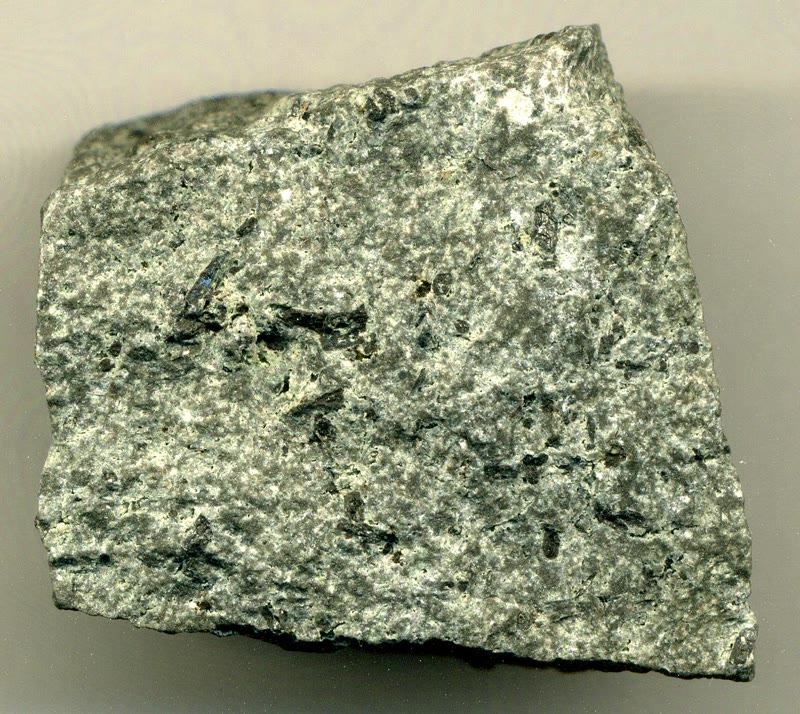
\includegraphics[height=4.4cm]{images/book2/g12-stjohn-andesite.jpg}\hspace{0.03\linewidth}%
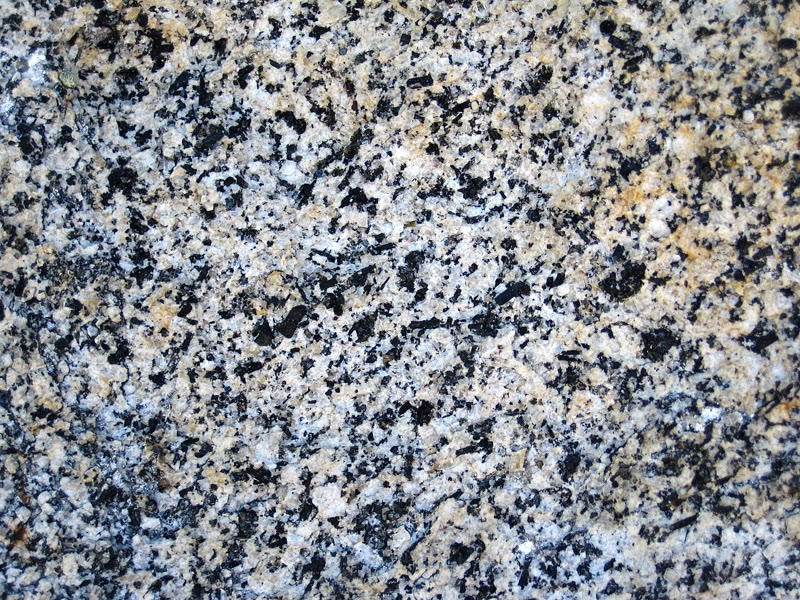
\includegraphics[height=4.4cm]{images/book2/g12-stjohn-granodiorite.jpg}

{\small Kiri: \omterm{def:g11:igneous-rocks:rock-names}{andesit}, \omterm{def:g11:igneous-rocks:volcanic-plutonic}{batuan vulkanik} berbutir halus dari busur. Kanan:
\omterm{def:g12:subduction-magmatism:granodiorite}{granodiorit} Sierra Nevada, dengan plagioklas putih, kuarsa kelabu, serta biotit
dan hornblende hitam. Foto James St.~John (CC~BY~2.0).}
\end{omfigure}
% ledger: photo:g12-andesite, photo:g12-granodiorite

Rata-rata, \omterm{def:g12:continental-crust:continental-crust}{kerak benua} bagian atas mengandung sekitar \qty{67}{\percent}
\ce{SiO2}: kerak itu \omterm{def:g11:igneous-rocks:felsic-mafic}{felsik}, seperti granit-granit yang dibuat busur dalam
jumlah besar di dalam \omterm{def:g12:subduction-magmatism:batholith}{batolit-batolitnya}.
% ledger: rg14:crust (upper crust SiO2 66.6 wt %), tulane:magma-types, tulane:intrusions

\begin{definition}[Batolit]\label{def:g12:subduction-magmatism:batholith}
Yang disebut \emph{batolit}\index{batolit} adalah massa \omterm{def:g11:igneous-rocks:volcanic-plutonic}{batuan plutonik} yang
besar yang menutupi lebih dari \qty{100}{km^2} di tempat erosi telah
menyingkapkannya. Batolit terbentuk di tempat banyak \omterm{def:g11:igneous-rocks:intrusion}{pluton}, yang menerobos
satu demi satu, bergabung di bawah permukaan.
\end{definition}
% ledger: earle:batholith, tulane:intrusions

Salah satu yang terbesar di dunia, Kompleks \omterm{def:g11:igneous-rocks:volcanic-plutonic}{Plutonik} Pesisir, membentang di
sepanjang pantai Pasifik dari wilayah Vancouver di Kanada barat sampai Alaska
tenggara. \omterm{def:g12:subduction-magmatism:batholith}{Batolit} Sierra Nevada di California terbentuk di atas \omterm{def:g11:subduction-zones:subduction}{zona subduksi};
sebagian besar granitnya di Yosemite mengkristal pada zaman Kapur, 105 sampai
85 juta tahun yang lalu. Batuan di atasnya terkikis selama jutaan tahun, dan
\omterm{def:g11:igneous-rocks:intrusion}{pluton-pluton} yang mendingin jauh di bawah itu kini membentuk pegunungan.
% ledger: earle:batholith, nps:yosemite, photo:g12-sierra-nevada (St. John description), ics:base.Cretaceous

\begin{omfigure}
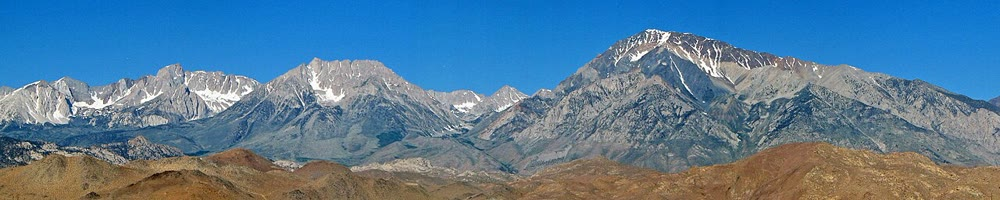
\includegraphics[width=0.94\linewidth]{images/book2/g12-stjohn-sierra-nevada-batholith.jpg}

{\small Sierra Nevada, dilihat dari timur: granit dan \omterm{def:g12:subduction-magmatism:granodiorite}{granodiorit} \omterm{def:g12:subduction-magmatism:batholith}{batolit}
Sierra Nevada, yang mengkristal jauh di bawah permukaan di atas \omterm{def:g11:subduction-zones:subduction}{zona subduksi}
pada zaman Kapur. Foto James St.~John (CC~BY~2.0).}
\end{omfigure}
% ledger: photo:g12-sierra-nevada, nps:yosemite

\section{Bagaimana benua tumbuh}

\begin{definition}[Pertumbuhan benua]\label{def:g12:subduction-magmatism:continental-growth}
Yang disebut \emph{pertumbuhan benua}\index{pertumbuhan benua} adalah
penambahan \omterm{def:g12:continental-crust:continental-crust}{kerak benua} baru, yang dibuat dari mantel, terutama oleh magmatisme
busur. Pertumbuhan bersih benua-benua adalah penambahan itu dikurangi \omterm{def:g12:continental-crust:continental-crust}{kerak
benua} yang kembali ke mantel.
\end{definition}
% ledger: sv09:growth, ss09:balance

Busur adalah tempat batuan ringan benua-benua dibuat. Perkiraan magma yang
ditambahkan busur saat ini adalah sekitar \qty{1.5}{km^3} setahun di busur
kepulauan dan \qty{1.0}{km^3} setahun di busur benua; dirata-ratakan dalam
jangka panjang, sekitar \qty{2.7}{km^3} setahun. Tetapi \omterm{def:g11:subduction-zones:subduction}{zona subduksi} juga
membawa kembali \omterm{def:g12:continental-crust:continental-crust}{kerak benua} ke dalam mantel: sedimen yang terbawa turun bersama
\omterm{def:g11:subduction-zones:slab}{lempengan} dan potongan-potongan lempeng yang berada di atas yang terkikis dari
bawah, sekitar \qty{3.2}{km^3} setahun. Keduanya berdekatan, dan pertumbuhan
bersih benua-benua selama beberapa ratus juta tahun terakhir mungkin nol, atau
bahkan negatif.
% ledger: sv09:growth, ss09:balance

Benua juga tumbuh di tepi-tepinya dengan cara lain. \omterm{def:g12:continental-crust:continental-crust}{Kerak benua} terlalu ringan
untuk tersubduksi, sehingga ketika sebuah lempeng membawa sebuah benua ke dalam
palung, kedua benua terlas bersama dalam sebuah tumbukan
(\cref{ch:g12:mountain-building}). Setiap benua mempunyai inti tua, sebuah
\omterm{def:g12:continental-crust:craton}{kraton}, yang dikelilingi sabuk-sabuk batuan yang lebih muda, yaitu \omterm{def:g12:continental-crust:root}{akar-akar}
terdeformasi dari sabuk-sabuk pegunungan masa lalu, yang ditambahkan satu demi
satu di tepi-tepinya (\cref{ch:g12:continental-crust}).
% ledger: tulane:no-subduct (continental crust too buoyant to subduct), earle:collision, tulane:cratons

\section{Latihan}

\begin{exercise}[$\star$]\label{exo:g12:subduction-magmatism:1}
Sebutkan istilahnya: (a) deretan gunung api yang sejajar dengan palung, pada
lempeng yang tidak tenggelam; (b) pelelehan yang disebabkan oleh penambahan air
pada sebuah batuan; (c) \omterm{def:g11:igneous-rocks:volcanic-plutonic}{batuan plutonik} dengan plagioklas yang lebih banyak
daripada feldspar kalium dan lebih dari \qty{20}{\percent} kuarsa; (d) massa
\omterm{def:g11:igneous-rocks:volcanic-plutonic}{batuan plutonik} yang lebih luas dari \qty{100}{km^2}; (e) penambahan \omterm{def:g12:continental-crust:continental-crust}{kerak benua}
baru yang dibuat dari mantel.
\end{exercise}

\begin{exercise}[$\star$]\label{exo:g12:subduction-magmatism:2}
Pada 18 Mei 1980 kolom abu Gunung St.~Helens naik lebih dari \qty{24}{km}
dalam waktu kurang dari 15 menit. (1) Berapa kecepatan naik rata-ratanya yang
terkecil, dalam \unit{km/h} dan dalam \unit{m/s}? (2) Bandingkan dengan
kecepatan semburan ke samping, setidaknya \qty{480}{km/h}.
\end{exercise}

\begin{exercise}[$\star$]\label{exo:g12:subduction-magmatism:3}
Dari 1214 gunung api dalam katalog yang aktif sejak akhir zaman es terakhir,
838 berdiri di atas \omterm{def:g11:subduction-zones:subduction}{zona subduksi}. (1) Berapa persen itu? (2) Di sisi palung
yang mana gunung-gunung api itu berada? (3) Mengapa tidak ada gunung api di
antara palung dan front vulkanik?
\end{exercise}

\begin{exercise}[$\star$]\label{exo:g12:subduction-magmatism:4}
Sebuah batuan berbutir kasar mengandung \qty{25}{\percent} kuarsa,
\qty{45}{\percent} plagioklas, \qty{15}{\percent} feldspar kalium, dan
\qty{15}{\percent} biotit dan hornblende. (1) Berapa bagian feldsparnya yang
berupa plagioklas? (2) Apakah batuan itu \omterm{def:g12:subduction-magmatism:granodiorite}{granodiorit}?
\end{exercise}

\begin{exercise}[$\star$]\label{exo:g12:subduction-magmatism:5}
Berikan dua alasan mengapa gunung api busur meletus lebih eksplosif daripada
gunung api punggungan.
\end{exercise}

\begin{exercise}[$\star\star$]\label{exo:g12:subduction-magmatism:6}
(1) Sebuah front vulkanik terletak \qty{150}{km} dari palungnya, di atas
\omterm{def:g11:subduction-zones:slab}{lempengan} yang miring \ang{35}. Seberapa dalam \omterm{def:g11:subduction-zones:slab}{lempengan} di bawahnya?
(2) Bandingkan dengan rata-rata \qty{105}{km}.
\end{exercise}

\begin{exercise}[$\star\star$]\label{exo:g12:subduction-magmatism:7}
Anggaplah \omterm{def:g11:subduction-zones:slab}{lempengan} terletak \qty{105}{km} di bawah setiap front vulkanik.
Seberapa jauh front itu dari palung bila \omterm{def:g11:subduction-zones:slab}{lempengan} miring \ang{20}, dan bila
miring \ang{45}? Apa yang dikatakan hal itu kepadamu tentang tempat mencari
busur?
\end{exercise}

\begin{exercise}[$\star\star$]\label{exo:g12:subduction-magmatism:8}
Pada \qty{100}{km}, tekanannya sekitar \qty{3.16}{GPa}. (1) Dengan $T =
-5.104P^2 + 132.9P + 1120.7$ ($P$ dalam \unit{GPa}, $T$ dalam \unit{\celsius}),
hitung suhu saat \omterm{def:g11:ocean-ridges:peridotite}{peridotit} kering mulai meleleh di sana. (2) Dengan air,
\omterm{def:g11:ocean-ridges:peridotite}{peridotit} mulai meleleh pada sekitar \qty{1000}{\celsius}. Berapa banyak air
menurunkannya? (3) Baji mantel di sana bersuhu, katakanlah,
\qty{1300}{\celsius}. Apakah baji itu meleleh dalam keadaan kering? Basah?
\end{exercise}

\begin{exercise}[$\star\star$]\label{exo:g12:subduction-magmatism:9}
Longsoran puing Gunung St.~Helens memindahkan sekitar \qty{2.5}{km^3} batuan.
Busur-busur menambahkan sekitar \qty{2.7}{km^3} kerak baru setahun. (1) Longsoran
itu setara dengan magmatisme busur sedunia selama berapa hari? (2) Mengapa
perbandingan itu hanya soal ukuran?
\end{exercise}

\begin{exercise}[$\star\star$]\label{exo:g12:subduction-magmatism:10}
(1) Berapa banyak kerak baru yang ditambahkan busur dalam sejuta tahun dengan
laju \qty{2.7}{km^3} setahun? (2) \omterm{def:g12:continental-crust:continental-crust}{Kerak benua} bervolume sekitar
\qty{9e9}{km^3}. Berapa lama busur saja memerlukan waktu untuk membuat volume
itu, bila tidak ada yang hilang? (3) Bandingkan dengan umur Bumi, 4.5 miliar
tahun.
\end{exercise}

\begin{exercise}[$\star\star$]\label{exo:g12:subduction-magmatism:11}
(1) Pada penampang yang melintasi Jepang, mengapa banyak gempa bumi yang lebih
dangkal dari \qty{70}{km} diabaikan ketika \omterm{def:g11:subduction-zones:slab}{lempengan} dicocokkan? (2) Gempa-gempa
dalam terletak pada kedalaman \qty{116}{km} di \ang{140.5}~BT dan \qty{80}{km}
di \ang{141.5}~BT, dengan \qty{86.4}{km} per derajat. Hitung kemiringan
\omterm{def:g11:subduction-zones:slab}{lempengan}.
\end{exercise}

\begin{exercise}[$\star\star\star$]\label{exo:g12:subduction-magmatism:12}
Tunjukkan bahwa, untuk front pada jarak $d$ dari palung di atas \omterm{def:g11:subduction-zones:slab}{lempengan} yang
kemiringannya $\theta$, jarak yang diukur menuruni \omterm{def:g11:subduction-zones:slab}{lempengan} dari palung sampai
titik di bawah front adalah $d/\cos\theta$. Untuk Jepang ($d = \qty{270}{km}$,
$\theta = \ang{20}$), berapa panjangnya? Lempeng Pasifik bergerak menuju
Jepang dengan laju sekitar \qty{83}{mm} setahun; dengan menganggap kecepatan
itu berlaku di sepanjang \omterm{def:g11:subduction-zones:slab}{lempengan}, berapa lama sepotong dasar laut menempuh
perjalanan dari palung sampai ke bawah gunung-gunung api?
\end{exercise}
% ledger: usgs:tohoku (83 mm/yr)

\begin{exercise}[$\star\star\star$]\label{exo:g12:subduction-magmatism:13}
Dapur magma Gunung St.~Helens selebar sekitar \qty{1}{km} dan membentang dari
kedalaman sekitar 6 sampai \qty{14}{km}. (1) Dengan menganggapnya sebagai
silinder tegak, perkirakan volumenya. (2) Bandingkan dengan \qty{2.5}{km^3}
longsoran itu. (3) Hitung \omterm{def:g12:metamorphic-rocks:lithostatic}{tekanan litostatik} di bagian atas dan bawahnya ($\rho =
\qty{2830}{kg/m^3}$, $g = \qty{9.81}{m/s^2}$).
\end{exercise}

\begin{exercise}[$\star\star\star$]\label{exo:g12:subduction-magmatism:14}
Busur-busur menambahkan sekitar \qty{2.7}{km^3} kerak setahun, dan \omterm{def:g11:subduction-zones:subduction}{zona
subduksi} membawa kembali sekitar \qty{3.2}{km^3}. (1) Berapa perubahan bersihnya
per sejuta tahun? (2) Selama 500 juta tahun, berapa bagian dari kerak yang
bervolume \qty{9e9}{km^3} jumlah itu? (3) Para penulisnya menyebut pertumbuhan
bersih itu ``praktis nol''. Mengapa, mengingat ketidakpastian setiap perkiraan?
\end{exercise}

\begin{exercise}[$\star\star\star$]\label{exo:g12:subduction-magmatism:15}
Sebuah \omterm{def:g12:subduction-magmatism:batholith}{batolit} menyingkapkan \omterm{def:g12:subduction-magmatism:granodiorite}{granodiorit} seluas \qty{20000}{km^2} yang
\omterm{def:g11:igneous-rocks:intrusion}{pluton-plutonnya} membeku pada kedalaman antara 5 dan \qty{15}{km}.
(1) Perkirakan volume magma yang diwakilinya, dengan menganggap tebalnya
\qty{10}{km}. (2) Dengan laju \qty{1}{km^3} setahun, laju seluruh busur benua
di dunia bersama-sama, berapa lama busur-busur itu memerlukan waktu untuk
membuatnya? Apa yang dikatakan hal itu kepadamu tentang waktu pembentukan
sebuah \omterm{def:g12:subduction-magmatism:batholith}{batolit}?
(3) Berapa banyak batuan yang harus terkikis dari atasnya sebelum \omterm{def:g12:subduction-magmatism:batholith}{batolit} itu
dapat terlihat?
\end{exercise}

\begin{problem}[{Soal akhir pekan --- Di bawah gunung-gunung api Jepang}]
\label{pb:g12:subduction-magmatism:1}
% ledger: data:b2-usgs-ne-japan, data:gvp, data:pb2002, sa06:slab-depth, hirschmann:solidus, wang20:wet-solidus, earle:arc-water, data:prem
% values (arc_magmatism.py): Megata 139.725, Iwate 141.001, trench 144.12; bins 140.5/141/141.5: 116.4/98.15/80.35 km; P_100km 3.157, dry_T_100km 1489
Gunung-gunung api Jepang timur laut antara \ang{37.5} dan \ang{40.5}~LU terletak
antara \ang{139.7}~BT (Megata, yang paling barat) dan \ang{141.0}~BT (Iwate, yang
paling timur); Palung Jepang terletak pada \ang{144.1}~BT. Tabel berikut
memberikan kedalaman median gempa-gempa bumi yang lebih dalam dari
\qty{70}{km} dalam tiga lajur bujur, 1976--2025. Ambillah \qty{111.2}{km} untuk
satu derajat lintang.

\begin{center}
\small
\begin{tabular}{|l|c|c|c|}
\hline
bujur (\unit{\degree}~BT) & 140.5 & 141.0 & 141.5 \\ \hline
kedalaman median (\unit{km}) & 116 & 98 & 80 \\ \hline
\end{tabular}
\end{center}

\medskip
\noindent\textbf{Bagian I --- Front vulkanik.}
\begin{enumerate}
  \item Tunjukkan bahwa satu derajat bujur pada \ang{39}~LU sekitar
        \qty{86.4}{km}.
  \item Seberapa jauh front vulkanik dari palung?
  \item Seberapa lebar busur itu, dari Iwate sampai Megata?
  \item Di atas lempeng mana gunung-gunung api itu berdiri, dan di sisi palung
        yang mana?
  \item Mengapa tidak ada gunung api di antara palung dan Iwate?
\end{enumerate}

\medskip
\noindent\textbf{Bagian II --- Penampang gempa bumi.}
\begin{enumerate}[resume]
  \item Berapa kilometer kedalaman median itu berubah dari \ang{140.5} sampai
        \ang{141.5}~BT?
  \item Pada jarak mendatar berapa?
  \item Hitung kemiringan \omterm{def:g11:subduction-zones:slab}{lempengan}.
  \item Teruskan garis dari \ang{141.0}~BT, \qty{98}{km}, ke atas sampai
        permukaan. Di mana garis itu mencapai permukaan, dan seberapa jauh
        tempat itu dari palung?
  \item Kemukakan mengapa \omterm{def:g11:subduction-zones:slab}{lempengan} itu kurang curam di dekat palung daripada
        di tempat yang lebih dalam.
\end{enumerate}

\medskip
\noindent\textbf{Bagian III --- Lempengan di bawah gunung-gunung api.}
\begin{enumerate}[resume]
  \item Hitung $H = d\tan\theta$ dengan jarak dari pertanyaan 2 dan kemiringan
        \ang{20}.
  \item Bandingkan dengan kedalaman median di bawah front.
  \item Bandingkan keduanya dengan rentang dunia, 72 sampai \qty{173}{km}, dan
        rata-ratanya, \qty{105}{km}.
  \item Seberapa dalam \omterm{def:g11:subduction-zones:slab}{lempengan} di bawah Megata, dengan garis dari
        pertanyaan 9?
  \item Dengan menganggap kerak busur setebal sekitar \qty{35}{km}, apakah
        bagian atas \omterm{def:g11:subduction-zones:slab}{lempengan} di bawah front berada di dalam kerak atau di dalam
        mantel? Seberapa jauh di bawah dasar kerak letaknya?
\end{enumerate}

\medskip
\noindent\textbf{Bagian IV --- Dari mana airnya berasal.}
\begin{enumerate}[resume]
  \item Di mana air \omterm{def:g11:subduction-zones:slab}{lempengan} itu masuk ke dalam batuannya, dan di dalam
        mineral apa sebagian besar air itu tersimpan?
  \item Pada \qty{100}{km} tekanannya sekitar \qty{3.16}{GPa}. Hitung solidus
        kering di sana dengan $T = -5.104P^2 + 132.9P + 1120.7$.
  \item Dengan air, solidusnya antara 950 dan \qty{1000}{\celsius}.
        Berapa banyak air menurunkannya?
  \item Mengapa \omterm{def:g11:subduction-zones:slab}{lempengan} yang dingin itu sendiri tidak dapat menjadi sumber
        magma?
  \item Simpulkan: seberapa dalam \omterm{def:g11:subduction-zones:slab}{lempengan} di bawah front vulkanik Jepang
        timur laut?
\end{enumerate}
\end{problem}
